\documentclass[12pt]{article}

\usepackage{mathrsfs}
\usepackage{epsfig}
\usepackage{graphicx}
\usepackage{color}
\usepackage{amsmath}
\usepackage{amsfonts}
\usepackage{amssymb}
\usepackage{amsthm}
\usepackage{amscd}
\usepackage{verbatim}
\usepackage{fullpage}
\usepackage{indentfirst}

%\setcounter{MaxMatrixCols}{20}
\theoremstyle{plain}
\newtheorem{theorem}{Theorem}[section]
\newtheorem{proposition}[theorem]{Proposition}
\newtheorem{lemma}[theorem]{Lemma}
\newtheorem{corollary}[theorem]{Corollary}
\newtheorem{conjecture}[theorem]{Conjecture}
\newtheorem{hypothesis}{Hypothesis}
\newtheorem{nullhypothesis}{Null Hypothesis}
\theoremstyle{definition}
\newtheorem{definition}[theorem]{Definition}
\newtheorem{notation}[theorem]{Notation}
\newtheorem{remark}[theorem]{Remark}
\newtheorem{example}[theorem]{Example}
\numberwithin{equation}{theorem}

\newcommand{\black}{\hfill{\ensuremath{\blacksquare}}}
\DeclareMathAlphabet{\mathpzc}{OT1}{pzc}{m}{it}

\graphicspath{ {./} }

\begin{document}
\begin{titlepage}
	\centering
	\vspace{4cm}
	{\scshape\Large DSE 210\par}
	\vspace{1.5cm}
	{\huge\bfseries Homework 5\par}
	\vspace{2cm}
	{\Large\itshape Kevin Kannappan\par}

% Bottom of the page
	{\large \today\par}
\end{titlepage}


\section{PCA and SVD}
\subsection{Worksheet 10}
\begin{enumerate}
\item The following set of vectors do not form an orthonormal basis of $\mathbb{R}^{3}$. The reasoning for why they do not is, while they are orthogonal and the dot products between each vector pair is 0, the first two vectors are not unit vectors. To be an orthonormal set of vectors, the vectors need to be both unit vectors and orthogonal.
\item Drew a rough sketch of ellipsoidal contours of the covariance matrices and the directions of the first and second eigenvectors directly on the plots. They can be viewed in the image below:
\bigskip
\begin{center}
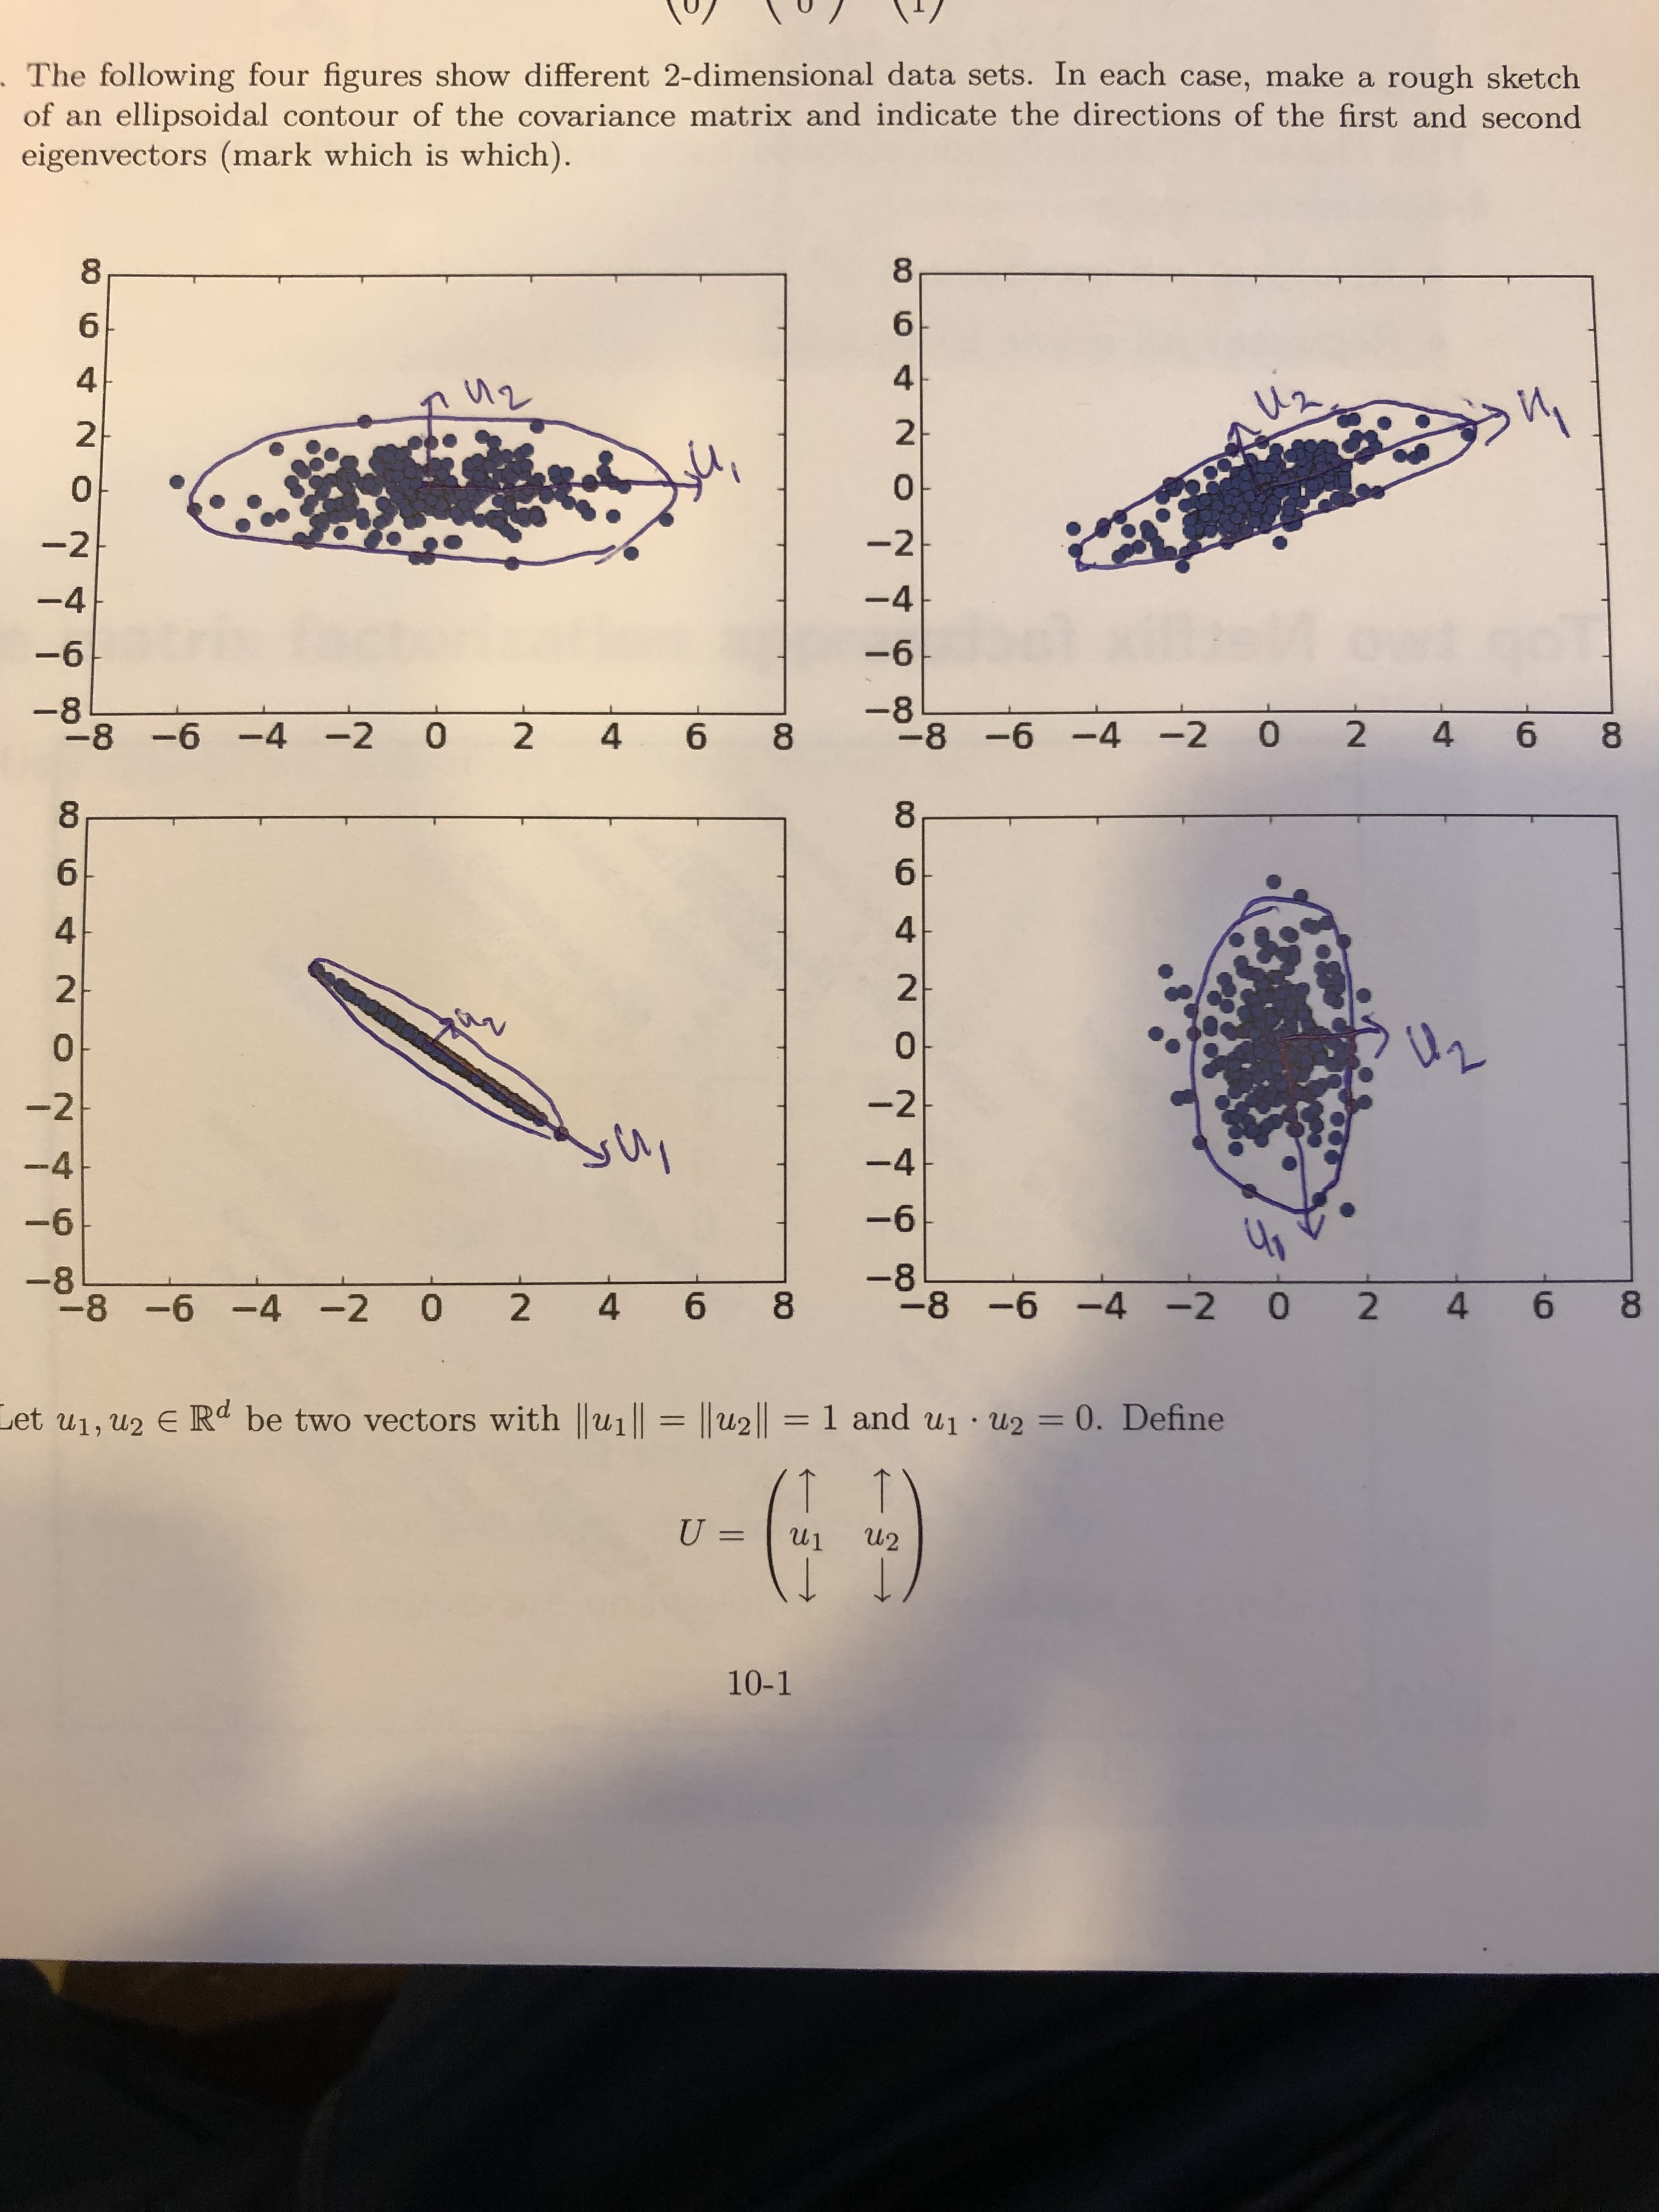
\includegraphics[width=9cm, height=12cm]{ws_10_q2}
\end{center}
\bigskip
\addtocounter{enumi}{2}
\item Please refer to Jupyter notebook for Problem 5.
\end{enumerate}
\bigskip

\section{Sampling}
\subsection{Worksheet 11}
\begin{enumerate}
\item The distribution of the number of red marbles seen, can be computed using the standard formula for $n$ tosses of a coin of bias $p$: $N(np,np(1-p))$. Substituting $n=900$ and $p=\frac{9}{10}$, we have:\\
\smallskip
$N(\frac{9}{10}*900,\frac{9}{10}*\frac{1}{10}*900)$\\
\smallskip
hence: $N(810,81)$, with $\mu = 810$ and $\sigma = 9$.
\item The distribution of the population of left-handedness, can be computed using the standard formula for $n$ tosses of a coin of bias $p$: $N(np,np(1-p))$. Substituting $n=200$ and $p=\frac{1}{100}$, we have:\\
\smallskip
$N(\frac{1}{100}*200,\frac{1}{100}*\frac{99}{100}*200)$\\
\smallskip
hence: $N(2,1.98)$, with $\mu = 2$ and $\sigma \approx 1.41$. To find the 99\% confidence interval for the number of people in the sample that are left handed, we take the mean and add/subtract 3 times the standard deviation: $2 \pm 3 \times 1.41$. The 99\% confidence interval is -2.23 to 6.23.
\addtocounter{enumi}{1}
\item Considering we have a population with 1\% colorblindness, then we have $n$ people at random, with the probability that none are colorblind at $0.99^{n}$. Since we want this probability of a sample to contain at least one colorblind person to be at least 95\%, then we just need to take the value for which $0.99^{n} < 0.05$. Computing on wolfram alpha, we find the real value to be 298. Hence, we must have a sample of at least 298 people to contain at least one person with probability 95\%.
\item Using the true fraction of San Diegans liking sushi of 0.5, we can leverage that $p=0.5$ for the distribution of the observed fraction of $n$ tosses of a coin of bias $p$: $N(np,\frac{p(1-p)}{n})$. The standard deviation is the square root of the variance, so we are solving for the second term, specifically: $\sqrt{\frac{p(1-p)}{n}}$:
	\begin{enumerate}
	\item For $n = 100$: $\sqrt{\frac{0.5^{2}}{100}} = 0.05$. $\sigma = 0.05$.
	\item For $n = 2500$: $\sqrt{\frac{0.5^{2}}{2500}} = 0.01$. $\sigma = 0.01$.
	\end{enumerate}
\item For this problem, $p$ is not provided. However, the good news is that $p$ at its largest variance (0.5) is also a reasonable estimate for the fraction of gender between males and females. For this problem we will set $p=0.5$ to calculate the sample size so that we can provide a confidence interval with confidence at least 99\% estimated within 0.01. Hence, we can solve for the value of $n$ such that $3*\sigma \leq 0.01$. Inserting $p=0.5$ into this forumula, we have:\\
\smallskip
$3*\sqrt{\frac{0.5^{2}}{n}} = 0.01$\\
\smallskip
$\sqrt{\frac{0.25}{n}} = \frac{0.01}{3}$ which is solved for n by wolfram alpha to be $\approx 22,500$, so maybe they could sample a small town in Wyoming.
\addtocounter{enumi}{1}
\item Using the observed proportion of people enrolled in college from ages 18-24, we have $p=0.388$. We can use this to solve for the estimate of the fraction of all persons age 18 to 24 in the city who are enrolled in college, we will also provide the 95.5\% confidence interval for the estimate, which is taken by multiplying by adding/subtracting $2*\sigma$ from the mean:\\
\smallskip
Since we are estimating the fraction of people 18 to 24 who are enrolled in college, we use the observed proportion to determine the mean. It is $p=0.388$. Or $\mu = 38.8\%$. To find the confidence interval, we need to solve for the standard deviation:\\
\smallskip
$0.388 \pm 2*(\sqrt{\frac{0.388*0.612}{500}})$, or\\
\smallskip
$0.388 \pm 2*0.02179$ which yields the 95\% confidence interval for the estimate of the mean between 34.4\% to 43.2\%.
\addtocounter{enumi}{1}
\item Using the observed average test score on the math component of the test for 17-year old students, we have $p=0.307$. We can use this to estimate the nationwide average score on the math test and compute the standard deviation of this estimate, using the sample standard deviation which was provided to be $\sigma = 30$.\\
\smallskip
Since we are estimating the nationwide average score on the math test, we use the observed proportion to determine the mean. It is $p=0.307$. Or $\mu = 307$. To find the standard deviation, we use the sample standard deviation:\\
\smallskip
The standard deviation is approximately $\frac{30}{\sqrt{1000}} \approx 0.95$. Hence, $\sigma=95$.
\end{enumerate}
\bigskip

\section{Hypothesis Testing}
\subsection{Worksheet 12}
\begin{enumerate}
\addtocounter{enumi}{1}
\item
	\begin{enumerate}
	\item Observational study.
	\item To avoid confounding effects.
	\item This should be tested in a controlled experiment, right now this is an observed effect that has yet to be studied further.
	\end{enumerate}
\addtocounter{enumi}{1}
\item No, it was not wise to let teachers to use their judgement in this way. Teachers are unable to randomly select students, hence the experiment was no longer random and thus the results are not valid.
\item Potentially, though I would expect it to be independent. The good news is there are ways to assess the validity and scope of this effect!
\item
	\begin{enumerate}
	\item
	\begin{nullhypothesis}The coin is fair\end{nullhypothesis}
	\begin{hypothesis}The coin is biased \end{hypothesis}
	\item Calculate mean: $\mu = 0.5*10000 = 5000$. Calculate standard deviation: $\sigma = \sqrt{10000*0.5^{2}} = 50$. Hence, $Z = \frac{5400-5000}{50} = 8$. Leveraging a Z-score table, we find the $p$-value to be $< 0.01$ which is statistically significant at the 99\% level.
	\item Since the $p$-value is statistically significant, we can safely reject the null hypothesis that the coin is fair and conclude that the coin is biased.
	\end{enumerate}
\item 	This can be explained as chance variation. Using mean and variance summation principles, we are able to conclude that the expected value is the same as the sum of the expected values, which is the same for the variance. Given that $\mu_{1} = 3.5$ and $\sigma_{1}^{2} \approx 2.7$, we just need to multiply the forumals by the amount of dice rolls (100). We can then determine the expected number of spots to be 350, which was given, and the variance to be $\approx 2742$. Hence, $\sigma \approx 52$, which would yield a $Z \approx 1$, which is not significant to reject the null hypothesis that the dice is fair.
\addtocounter{enumi}{1}
\item
	\begin{enumerate}
	\item $\sigma_{1} = \sqrt{\frac{0.219*0.781}{700}} \approx 0.01563$, $\sigma_{2} = \sqrt{\frac{0.11*0.89}{700}} \approx 0.01183$. Hence, $\sigma = \sqrt{0.01563^{2}+0.01183^{2}} \approx 0.01960$. From here, we calculate $Z=\frac{0.219-0.11}{0.01960} \approx 5.6$. The difference in marijuana usage percentage is real.
	\item $\sigma_{1} = \sqrt{\frac{0.369*0.631}{700}} \approx 0.01824$, $\sigma_{2} = \sqrt{\frac{0.11*0.89}{700}} \approx 0.01762$. Hence, $\sigma = \sqrt{0.01824^{2}+0.01762^{2}} \approx 0.02536$. From here, we calculate $Z=\frac{0.369-0.319}{0.02536} \approx 1.97$. The difference in cigarette smoking percentage is real.
	\end{enumerate}
\item $\sigma_{pu} = \frac{10.5}{\sqrt{1000}} \approx 0.3320$, $\sigma_{pr} = \frac{9.9}{\sqrt{1000}} \approx 0.3131$. Hence, $\sigma = \sqrt{0.3320^{2}+0.3131^{2}} \approx 0.4564$. From here, we calculate $Z=\frac{12.2-9.2}{0.4564} \approx 6.6$. The difference in working hours between public and private universities is extremely unlikely to be due to chance.
\end{enumerate}
\bigskip

\end{document}